\documentclass[12pt,onecolumn]{article}
\usepackage{listings}
\usepackage{float}
\usepackage{mathtools}
\usepackage{hyperref}
\usepackage[russian]{babel}
\everymath{\displaystyle}
\usepackage{placeins}
\usepackage[table,xcdraw]{xcolor}
\usepackage{geometry}
\geometry{
  a4paper,
  top=25mm, 
  right=15mm, 
  bottom=25mm, 
  left=15mm
}

\begin{document}
\setcounter{tocdepth}{4}
\begin{center}
    Санкт-Петербургский Национальный Исследовательский\\ 
    Университет ИТМО\\
    Мегафакультет Компьютерных Технологий и Управления\\
    Факультет Программной Инженерии и Компьютерной Техники \\
    
\includegraphics[scale=0.3]{itm.jpg} % нужно закинуть картинку логтипа в папку с отчетом
\end{center}
\vspace{1cm}


\begin{center}
    \large \textbf{Вариант №311678876767}\\
    \textbf{Лабораторная работа №3}\\
    по дисциплине\\
    \textbf{Программирование}
\end{center}

\vspace{2cm}

\begin{flushright}
  Выполнил Студент  группы P3116\\
  \textbf{Алексей Лапин}\\
  Преподаватель: \\
  \textbf{Сорокин Роман Борисович}\\
\end{flushright}

\vspace{10cm}
\begin{center}
    г. Санкт-Петербург\\
    2021г.
\end{center}
\newpage
\tableofcontents
\newpage
\section{Текст задания}
\textbf{Программа должна удовлетворять следующим требованиям:}
\begin{itemize}
  \item Доработанная модель должна соответствовать принципам SOLID.
  \item Программа должна содержать как минимум два интерфейса и один абстрактный класс (номенклатура должна быть согласована с преподавателем).
  \item В разработанных классах должны быть переопределены методы equals(), toString() и hashCode().
  \item Программа должна содержать как минимум один перечисляемый тип (enum).
\end{itemize}
\textbf{Порядок выполнения работы:}
\begin{itemize}
  \item Доработать объектную модель приложения.
  \item Перерисовать диаграмму классов в соответствии с внесёнными в модель изменениями.
  \item Согласовать с преподавателем изменения, внесённые в модель.
  \item Модифицировать программу в соответствии с внесёнными в модель изменениями.
\end{itemize}
\textbf{Описание предметной области, по которой должна быть построена объектная модель:}\\
Нужно сказать, что Незнайка никогда не забывал о своем больном друге. Не проходило дня, чтоб он не забежал к нему хотя бы на минутку. Обычно это удавалось сделать во время послеобеденной прогулки. Всегда, когда Незнайка обедал с собаками, он не съедал свою порцию до конца, а припрятывал в карман то пирожок, то котлетку, то хлебца краюшку и относил все это голодному Козлику. В первый же день он обратился к госпоже Миноге с просьбой заплатить ему жалованье хотя бы за недельку вперед, так как ему нужно помочь больному приятелю, который находился в дрянингской ночлежке. Госпожа Минога сказала, что теперь он живет в богатом доме, в обществе приличных собак, и ему не пристало водить компанию с каким-то Козликом, который даже дома собственного не имеет, а обитает в какой-то ночлежке.
\newpage
\section{Диаграмма классов объектной модели.}
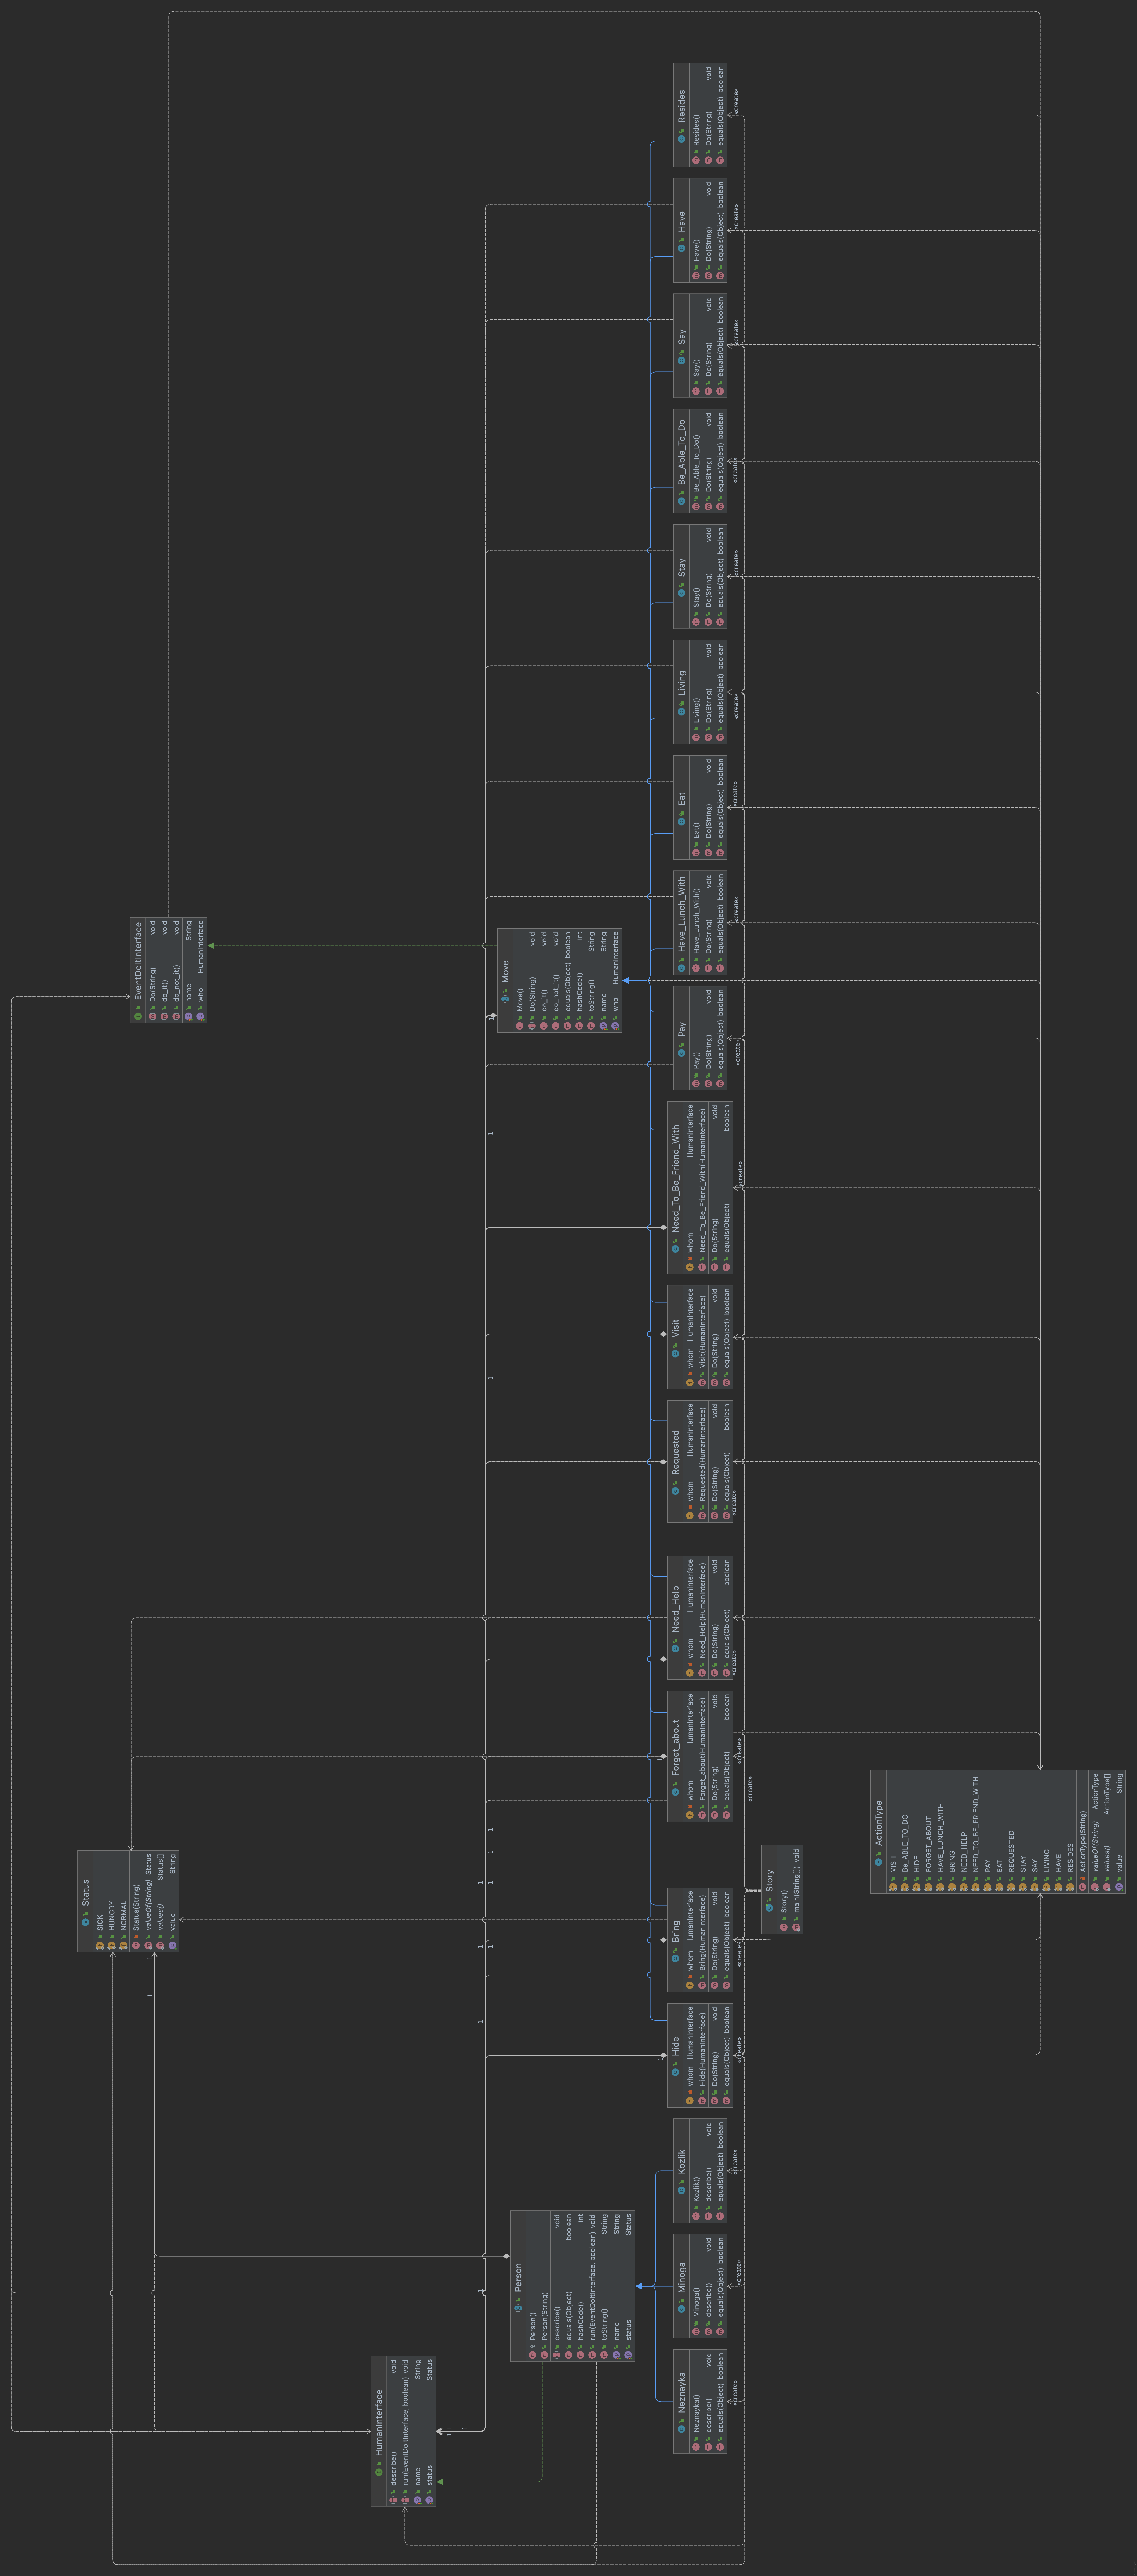
\includegraphics[scale=0.07]{UML.png}
\section{Исходный код программы}
\lstloadlanguages{Java}
\definecolor{mygray}{RGB}{120,120,120}
\lstset{extendedchars =/true,
breaklines=true,
basicstyle=\ttfamily\fontsize{9pt}{9pt}\selectfont,
commentstyle=\color{mygray},
keywordstyle=\color{blue},
}
Story.java
\lstinputlisting[language=Java,numbers=left]{Story.java}
Status.java
\lstinputlisting[language=Java,numbers=left]{Status.java}
people\\
HumanInterface.java
\lstinputlisting[language=Java,numbers=left]{people/HumanInterface.java}
Kozlik.java
\lstinputlisting[language=Java,numbers=left]{people/Kozlik.java}
Minoga.java
\lstinputlisting[language=Java,numbers=left]{people/Minoga.java}
Neznayka.java
\lstinputlisting[language=Java,numbers=left]{people/Neznayka.java}
Person.java
\lstinputlisting[language=Java,numbers=left]{people/Person.java}
event\\
ActionType.java
\lstinputlisting[language=Java,numbers=left]{event/ActionType.java}
EventDoItInterface.java
\lstinputlisting[language=Java,numbers=left]{event/EventDoItInterface.java}
Move.java
\lstinputlisting[language=Java,numbers=left]{event/Move.java}
Be\_Able\_To\_Do.java
\lstinputlisting[language=Java,numbers=left]{event/Be_Able_To_Do.java}
Bring.java
\lstinputlisting[language=Java,numbers=left]{event/Bring.java}
Eat.java
\lstinputlisting[language=Java,numbers=left]{event/Eat.java}
Forget\_about.java
\lstinputlisting[language=Java,numbers=left]{event/Forget_about.java}
Have\_Lunch\_With.java
\lstinputlisting[language=Java,numbers=left]{event/Have_Lunch_With.java}
Hide.java
\lstinputlisting[language=Java,numbers=left]{event/Hide.java}
Have.java
\lstinputlisting[language=Java,numbers=left]{event/Have.java}
Living.java
\lstinputlisting[language=Java,numbers=left]{event/Living.java}
Need\_Help.java
\lstinputlisting[language=Java,numbers=left]{event/Need_Help.java}
Need\_To\_Be\_Friend\_With.java
\lstinputlisting[language=Java,numbers=left]{event/Need_To_Be_Friend_With.java}
Pay.java
\lstinputlisting[language=Java,numbers=left]{event/Pay.java}
Requested.java
\lstinputlisting[language=Java,numbers=left]{event/Requested.java}
Resides.java
\lstinputlisting[language=Java,numbers=left]{event/Resides.java}
Say.java
\lstinputlisting[language=Java,numbers=left]{event/Say.java}
Stay.java
\lstinputlisting[language=Java,numbers=left]{event/Stay.java}
Visit.java
\lstinputlisting[language=Java,numbers=left]{event/Visit.java}
\section{Результат выполнения:}
\tiny{
\begin{verbatim}
На сцене появился Незнайка
На сцене появился Козлик
Статус персонажа Козлик изменён на SICK
Незнайка никогда не забывал о своем больном друге Козлике.
Не проходило дня, чтоб Незнайка не забежал к Козлику хотя бы на минутку.
Обычно это удавалось сделать во время послеобеденной прогулки.
Всегда, когда Незнайка обедал с собаками,
Незнайка не съедал свою порцию до конца,
а припрятывал в карман то пирожок, то котлетку, то хлебца краюшку
Статус персонажа Козлик изменён на HUNGRY
и относил все это голодному Козлику.
На сцене появилась госпожа Минога
В первый же день Незнайка обратился к Госпожа Минога
с просьбой заплатить Незнайке жалованье хотя бы за недельку вперед,
так как Незнайке нужно помочь голодному Козлику
Козлик находился в дрянингской ночлежке.
Госпожа Минога сказала,
что теперь Незнайка живёт в богатом доме, в обществе приличных собак,
и Незнайке не пристало водить компанию с каким-то Козликом,
Козлик даже дома собственного не имеет,
а обитает в какой-то ночлежке.
\end{verbatim}
}
\section{Вывод}
\normalsize
В процессе выполнения этой лабораторной работы я познакомился с принципами SOLID.
Познакомился с интерфейсами и абстрактными классами в языке Java.
\end{document}